\documentclass[a4paper, 11pt]{article} % Font size (can be 10pt, 11pt or 12pt) and paper size (remove a4paper for US letter paper)
\usepackage{helvet}
\renewcommand{\familydefault}{\sfdefault}
\usepackage[protrusion=true,expansion=true]{microtype} % Better typography
\usepackage{graphicx} % Required for including pictures
\usepackage[usenames,dvipsnames]{color} % Coloring code
\usepackage{wrapfig} % Allows in-line images
\usepackage[utf8]{inputenc}
\usepackage{enumerate}
\usepackage{enumitem}
\usepackage{framed, color}
\definecolor{shadecolor}{rgb}{0.690, 0.933, 0.525}

% Imágenes
\usepackage{graphicx} 

\usepackage{amsmath}
% para importar svg
%\usepackage[generate=all]{svgfig}

% sudo apt-get install texlive-lang-spanish
\usepackage[spanish]{babel} % English language/hyphenation
\selectlanguage{spanish}
% Hay que pelearse con babel-spanish para el alineamiento del punto decimal
\decimalpoint
\usepackage{dcolumn}
\newcolumntype{d}[1]{D{.}{\esperiod}{#1}}
\makeatletter
\addto\shorthandsspanish{\let\esperiod\es@period@code}
\makeatother

\usepackage{longtable}
\usepackage{tabu}
\usepackage{supertabular}

\usepackage{multicol}
\newsavebox\ltmcbox

% Para algoritmos
\usepackage{algorithm}
\usepackage{algorithmic}
\usepackage{amsthm}

% Para matrices
\usepackage{amsmath}

% Símbolos matemáticos
\usepackage{amssymb}
\usepackage{accents}
\let\oldemptyset\emptyset
\let\emptyset\varnothing

\usepackage[hidelinks]{hyperref}

\usepackage[section]{placeins} % Para gráficas en su sección.
\usepackage[T1]{fontenc} % Required for accented characters
\usepackage{tikz}
\newenvironment{allintypewriter}{\ttfamily}{\par}
\setlength{\parindent}{0pt}
\parskip=8pt
\linespread{1.05} % Change line spacing here, Palatino benefits from a slight increase by default

\makeatletter
\renewcommand\@biblabel[1]{\textbf{#1.}} % Change the square brackets for each bibliography item from '[1]' to '1.'
\renewcommand{\@listI}{\itemsep=0pt} % Reduce the space between items in the itemize and enumerate environments and the bibliography
\newcommand{\imagen}[2]{\begin{center} \includegraphics[width=90mm]{#1} \\#2 \end{center}}
\newcommand{\RFC}[1]{\href{https://www.ietf.org/rfc/rfc#1.txt}{RFC-#1}}

\renewcommand{\maketitle}{ % Customize the title - do not edit title and author name here, see the TITLE block below
\begin{center} % Center align
{\Huge\@title} % Increase the font size of the title
\end{center}

\vspace{20pt} % Some vertical space between the title and author name

\begin{flushright} % Right align
{\large\@author} % Author name
\\\@date % Date

\vspace{40pt} % Some vertical space between the author block and abstract
\end{flushright}
\renewcommand{\baselinestretch}{0.5}

}


\usepackage[a4paper]{geometry}
\geometry{top=2cm, bottom=2cm, left=2.25cm, right=2.25cm}

%----------------------------------------------------------------------------------------
%	TITLE
%----------------------------------------------------------------------------------------

\title{\textbf{Computación, Machine Learning}\\ % Title
\vspace{20 pt}
Historia de las Matemáticas} % Subtitle

\author{\textsc{Daniel López García\\
Lothar Soto Palma\\
Elena Toro Pérez} % Author
\\{\textit{Universidad de Granada}}} % Institution

\date{\today} % Date

\newcounter{ndef}

\begin{document}
	\maketitle
	\tableofcontents
	\listoffigures
	\newpage
\section{Introduccion}
\textbf{Machine learning} es una disciplina científica del ámbito de la Inteligencia Artificial que crea sistemas que aprenden automáticamente.

Pero, ¿qué significan las palabras aprender y automáticamente, en este contexto?

\textit{Aprender} en este contexto quiere decir identificar patrones complejos en millones de datos. La máquina que realmente aprende es un algoritmo que revisa los datos y es capaz de predecir comportamientos futuros. 

\textit{Automáticamente}, también en este contexto, implica que estos sistemas se mejoran de forma autónoma con el tiempo, sin intervención humana.

Hoy en día, podemos observar la aplicación concreta de Machine Learning en varios campos que nos rodean, como son:
		\begin{itemize}
		    \item \textbf{Automóviles:} Sistemas de piloto automático, Detección de fallos por reconocimiento externo de vibraciones...
		    \item \textbf{Bancos:} Lectura de cheques y otros documentos, Detección de fraude en transacciones...
		    \item \textbf{Electrónica:} Reconocimiento de voz, visión artificial...
		    \item \textbf{Finanzas:} Asesoría de préstamos (aceptación/denegación de un crédito), Identificación de falsificaciones, Interpretación y reconocimiento de firmas...
		    \item \textbf{Internet:} Compras on-line, Anuncios on-line, Selección de clientes potenciales basándose en comportamientos en las redes sociales, interacciones en la web...
		    \item \textbf{Manufactura:}  Inspección de calidad mediante sistemas visuales, Control de la producción y del proceso, Análisis y diseño de productos....
		    \item \textbf{Medicina:} Análisis de células portadoras de cáncer mamario, Diseño de prótesis, Diseño de prediagnósticos médicos basados en síntomas del paciente...
		    \item \textbf{Recursos Humanos:} Predicción de qué empleados serán más rentables el año que viene.
		    \item \textbf{Robótica:} Control dinámico de trayectoria, Sistemas ópticos...
		    \item \textbf{Seguridad:} Reconocimiento de huellas digitales, Criptografía...		\item \textbf{Telecomunicaciones:} Compresión de datos e imágenes, Automatización de servicios de información, Decidir cuál es la mejor hora para llamar a un cliente...
		    \item \textbf{Transporte:} Sistemas de rutas y seguimiento de flotas, Diagnóstico de frenos en camiones...
		    \item \textbf{Voz:} Reconocimiento de voz, Transformación de texto escrito a voz...
		\end{itemize}
		
\underline{Un ejemplo concreto} de aplicación de esta técnica puede ser el siguiente:

\begin{shaded}
Una empresa de telefonía quiere saber qué clientes están en “peligro” de darse de baja de sus servicios para hacer acciones comerciales que eviten que se vayan a la competencia.

¿Cómo puede hacerlo? La empresa tiene muchos datos de los clientes, pero seguramente los usa solo para facturar y para hacer estadísticas.

¿Qué más puede hacer con esos datos? Se pueden usar para predecir cuándo un cliente se va a dar de baja y gestionar la mejor acción que lo evite.

Los datos históricos del conjunto de los clientes, debidamente organizados y tratados en bloque, generan una base de datos que se puede explotar para predecir futuros comportamientos (favorecer aquellos que mejoran los objetivos de negocio y evitar aquellos que son perjudiciales).

Esa cantidad inmensa de datos son imposibles de analizar por una persona para sacar conclusiones y menos todavía para hacer predicciones. Los algoritmos en cambio sí pueden detectar patrones de comportamiento contando con las variables que le proporcionamos y descubrir cuáles son las que han llevado, en este caso, a darse de baja como cliente.
\end{shaded}

\begin{figure}[H]
\centering
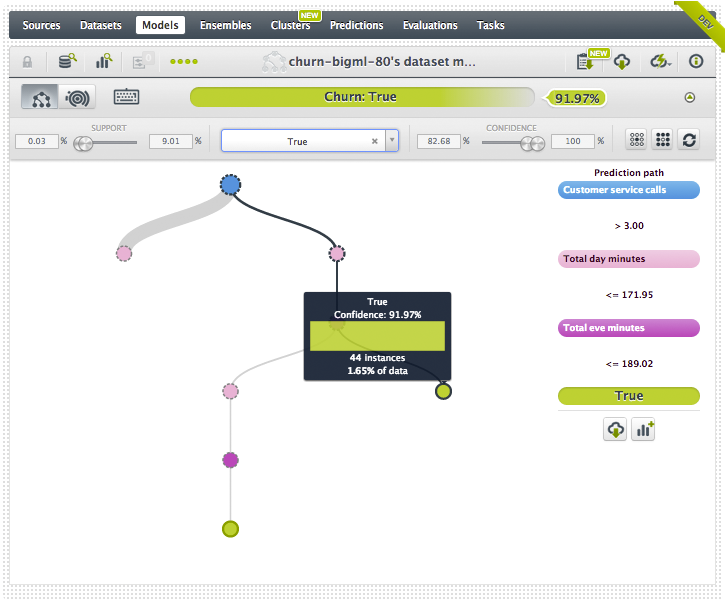
\includegraphics[width=0.95\textwidth]{ejemploMachineLearning.png}
\caption{Ejemplo de una predicción simplificada basada en datos de una compañía de telefonía ficticia, pero usando una herramienta de Machine Learning real}
\label{Ejemplo de una predicción simplificada basada en datos de una compañía de telefonía ficticia, pero usando una herramienta de Machine Learning real}
\end{figure}


\begin{shaded}
La visualización en árbol (en esta imagen está simplificado) permite ver los patrones que han seguido ciertos clientes que se han dado de baja.

En este caso está resaltada una de las ramas centrales, que indican un patrón en el que el cliente:
\begin{itemize}
    \item Tiene más de $3$ llamadas al servicio de atención al cliente.
    \item Llama menos de $171,95$ minutos al día.
    \item Las llamadas en horario nocturno son inferiores a $189,02$ minutos.
\end{itemize}

Por tanto, la predicción sería: \textit{Si los clientes que tienen estas características ya se han dado de baja de la compañía, es previsible que los que todavía son clientes y tienen este mismo comportamiento estén en riesgo de irse. Según este modelo predictivo, es bastante probable que esto suceda (se dice que la predicción tiene una confianza, en este caso, del $91,97\%$).}

Si el departamento de marketing tuviera esta información, podría proponerles a dichos clientes un cambio de plan de tarificación o podría revisar por qué han llamado al servicio de atención al cliente para intentar mantenerlos.
\end{shaded}
\section{Linea temporal}

\newpage

\section{Antecedentes estadísticos}
El machine learning 
\begin{itemize}
	\item \textbf{Teorema de Bayes:}. En 1812 \textbf{Pierre-Simon Laplace} publica \emph{Théorie Analytique des Probabilités}, en la que expande la obra de Bayes y define lo que ahora se conoce como Teorema de Bayes.
	
	\begin{figure}[H]
		\centering
		
\includegraphics[width=0.3\textwidth]{bayes.png}
		\caption{Teorema de Bayes}
		\label{Teorema de Bayes}
	\end{figure}

	La teoría bayesiana es muy usada en machine learning. Su básica idea es que todo lo que has aprendido es incierto, así que tienes que calcular la probabilidad de que sea incorrecto, e ir actualizándola según las pruebas. De acuerdo a estos principios se crearon los primeros filtros de correo spam.
	
	\item \textbf{Método de los mínimos cuadrados}.Adrien-Marie Legendre describió en \textbf{1805} el \emph{"méthode des moindres carrés"} conocida como el método de los mínimos cuadrados.
	
	Su aplicación más importante es en ajuste de datos. El mejor ajuste en el sentido de los mínimos cuadrados minimiza la suma de los residuos cuadrados, siendo un residuo la diferencia entre un valor observado y el valor ajustado proporcionado por un modelo.
	\item \textbf{Cadenas de Markov:} En \textbf{1948 Claude Shannon} publicó un artículo, \emph{The Mathematical Theory of Communication}, en el que creó el campo de la teoría de la información, introduciendo el concepto de entropía a través del modelado de Markov del inglés. Estos modelos idealizados pueden capturar muchas de las regularidades estadísticas de los sistemas. También permiten una estimación efectiva del estado y reconocimiento de patrones.
	
\end{itemize}
\section{Máquina de aprendizaje de Turing}
\textbf{Alan Turing} (1912-1954) fue un matemático, criptógrafo, filósofo y un teórico de la computación que, además de trabajar en el equipo que descifró los códigos Enigma de Alemania, fue un pionero en el campo de la inteligencia artificial publicando uno de los primeros trabajos sobre esta materia.

En \textbf{1950}, Alan Turing publicó uno de sus artículos más importantes para la revista \textit{Mind} (y que está considerado como una de las piedras angulares de la inteligencia artificial), \textit{Computing Machinery and Intelligence}, donde propuso un experimento: \textbf{el Test de Turing}.

El Test de Turing se basa en una hipótesis positivista que parte del principio de que "si una máquina se comporta en todos los aspectos como inteligente, entonces, dicha máquina debe ser inteligente".

El artículo de Turing comenzaba con una frase que era toda una declaración de intenciones de lo que evaluaría el test:
\begin{shaded}
"Propongo considerar la siguiente cuestión: ¿Pueden pensar las máquinas?"
\end{shaded}

Por lo que el resultado que se obtiene de este test es intentar medir si una máquina puede ser inteligente con un método que, aún hoy, sigue estando vigente.\\

La incógnita sobre la capacidad de las máquinas de pensar tiene una larga historia, esta se divide entre las perspectivas materialista y dualista de la mente.

Veamos algunos antecedentes al Test de Turing:
\begin{itemize}
    \item \textbf{René Descartes} tuvo ideas similares a la prueba de Turing en su texto \textit{Discurso del Método} de \textbf{1637} donde escribió: "\textit{Cuántos autómatas diferentes o máquinas móviles se pueden construir por la industria del hombre […] Podemos comprender con facilidad el hecho de que una máquina sea diseñada para pronunciar palabras, incluso responder ante acciones tangibles que produzcan un cambio en sus órganos; por ejemplo, si se le tocara de una manera particular no preguntaría qué le queremos decir; si se le toca en otra parte puede decir que se le está lastimando entre otras cosas. Pero nunca sucede que pueda ordenar su habla en distintas maneras para responder apropiadamente ante todo lo que se diga en su presencia, de la misma manera que la clase más baja de humanos puede hacerlo.}"
    
    Descartes reconoce que los autómatas son capaces de reaccionar ante interacciones humanas, pero argumenta que tal autómata carece de la capacidad de responder adecuadamente ante lo que se diga en su presencia, de la misma manera en la que un humano podría.
    
    Por lo tanto, Descartes abre las puertas para la prueba de Turing al identificar la insuficiencia de una respuesta lingüística apropiada, lo cual separa al humano del autómata. Descartes no llega a considerar que una respuesta lingüística apropiada puede ser producida por un autómata del futuro y, por lo tanto, no propone el test de Turing como tal, aunque ya razonó los criterios y el marco conceptual.
    
    \item \textbf{Denis Diderot} también planteó, en su \textit{Pensées philosophiques}, un criterio de la prueba de Turing: "\textit{Si se encuentra un loro que puede responder a todo, se le consideraría un ser inteligente sin duda alguna.}"
    
    Aunque esto no signifique del todo que él esté de acuerdo con el posterior Test de Turing, sí muestra que ya era un argumento común usado por los materialistas de la época.
    
    \item En \textbf{1936}, el filósofo \textbf{Alfred Ayer} consideraba la pregunta filosófica típica sobre otras mentes: "\textit{¿Cómo sabemos que otras personas experimentan el mismo nivel de conciencia que nosotros?.}"
    
    En su libro \textit{Lenguaje, Verdad y Lógica}, Ayer propuso un método para distinguir entre un hombre consciente y una máquina inconsciente: "\textit{El único argumento que tengo para asegurar que, lo que parece ser consciente, no es un ser consciente sino un muñeco o una máquina, es el hecho de que falle en las pruebas empíricas por medio de las cuales se determina la presencia o ausencia de la conciencia}". O, lo que es lo mismo, "\textit{algo no está consciente si reprueba una prueba de consciencia}".
    
    Esta es una propuesta muy similar a la prueba de Turing, aunque esta se enfoca en la conciencia en vez de en la inteligencia. Además se desconoce si Turing estaba familiarizado con el clásico filosófico de Ayer.\\ 
\end{itemize}

\textbf{¿En qué consistía el Test de Turing?} El Test de Turing se basaba en el Juego de la Imitación, una prueba en la que se ubicaban en una habitación un \textbf{hombre} y a una \textbf{mujer} frente a terminales que tuviesen algún sistema de comunicación (teletipos en los años 50).

En otra habitación, estando aislado, se encontraba un sujeto bajo estudio que actuaba como \textbf{interrogador}. Este último debía averiguar quién era el hombre y quién era la mujer, simplemente, con preguntas en lenguaje natural (escribiendo en un lenguaje que todos entendían).

El objetivo del interrogador era descubrir quién era la mujer y quién era el hombre, mientras que el de los otros dos era convencer al interrogador de que son la mujer.

Turing proponía realizar un cambio en este juego: coger a uno de los dos sujetos y sustituirlo por una \textbf{máquina}. Así, Turing cambiaba el objetivo de reconocer el sexo por el de reconocer la máquina.

\begin{figure}[H]
\centering
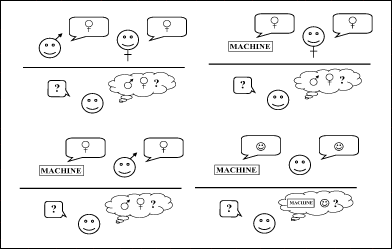
\includegraphics[width=0.52\textwidth]{testdeturing.PNG}
\caption{Test de Turing}
\label{Test de Turing}
\end{figure}

 La finalidad de estos cambios era hacer el juego lo más justo posible.
 \begin{enumerate}
     \item Lo primero, era que no tenía que consistir en un concurso de engaños, por lo que uno de los implicados no tendría por qué aparentar ser otra cosa.
     \item Otro detalle es que a Turing poco le importaba si el ordenador empleaba trucos preestablecidos para eludir o manipular las respuestas (por ejemplo, equivocándose en preguntas aritméticas o tardando más tiempo del necesario en responderlas). Suponía que el interrogador también las empleaba para reconocerle, así que lo importante era lo que resultaba del juego, no los métodos que se empleaban para jugar ni los mecanismos internos de razonamiento, que, entre otras cosas, también eran desconocidos en el ser humano.
 \end{enumerate}

Dado que el interrogador era humano, la máquina debería ser capaz de responder, inteligentemente, a cualquiera de las cuestiones que se le planteasen. Si la máquina era lo suficientemente hábil, el interrogador no podría distinguir quién era la máquina y quién el ser humano.

\begin{shaded}
Pero, "¿puede una máquina responder con un lenguaje natural a cualquier pregunta planteada por el interrogador?" "¿Puede pensar una máquina?"
\end{shaded}

Esas son las grandes preguntas que Turing plantea en este experimento. Lógicamente, salvo que una máquina emita sonidos que imiten la voz humana, la mejor manera de realizar la prueba es mediante lenguaje escrito y evaluar, únicamente, la inteligencia del oponente y la "humanidad" de las respuestas obtenidas a las preguntas planteadas.

Para que una máquina pudiese pasar el Test de Turing, ésta tendría que ser capaz de realizar las tareas para las que fue programada y, además, aprender por sí misma a realizar otras funciones.

Se dice que una máquina podría pasar el Test de Turing cuando el interrogador no lograra reconocerlo en un número significativo de ocasiones.

Hoy en día, estamos acostumbrados a ver algunos mecanismos que se apoyan en el Test de Turing, por ejemplo, los \textit{Captchas} (\textit{Completely Automated Public Turing Test to tell Computers and Humans Apart}) que aunque no son un test de Turing puro, se utilizan en muchas páginas web para evitar que procesos automatizados puedan registrar usuarios falsos o escribir mensajes de spam.

\section{La red neuronal en el tiempo}
Las \textbf{redes neuronales} son un conjunto de neuronas artificiales interconectadas, son un paradigma de aprendizaje y procesamiento automático inspirado en el sistema nervioso, que es objeto de estudio en el campo de la inteligencia artificial, pero \textbf{¿Cuándo surgió esta idea?} y \textbf{¿Qué ideas han dado lugar a las redes neuronales tal y como son en la actualidad?}.

En el año \textbf{1943}, el neurofisiólogo \textbf{Warren McCulloch} y el matemático \textbf{Walter Pitts} escribieron un documento en el que se describe como podrían funcionar las neuronas construyendo un modelo simple de red neuronal usando circuitos electrónicos. Para esto se basan en dos puntos de vista distintos, los procesos biológicos del cerebro y la aplicación de estas redes en la inteligencia artificial.

En el año \textbf{1949} \textbf{Donald Hebb} en su obra '\textit{'The Organization of Behavior''} señala el hecho de que cada vez que se usa un camino de una red neuronal estas se fortalecen explicando que este concepto es fundamental para el aprendizaje de un ser humano y esto es conocido como regla de hebb o teoría de la asamblea celular. Este es un mecanísmo de plasticidad sináptica (que se encarga de la modulación de percepción se estimulos de una neurona) en el que el valor de una conexión sináptica se incrementa si las neuronas de ambos lados de dicha sinapsis se activan repetidas veces de forma simultanea, la teoria suele resumirsa a la frase: "Las células que disparan juntas, permanecerán conectadas", aunque esta no debe tomarse literalmente. Esta forma de aprendizaje se denomina \textbf{aprendizaje de Hebb} o \textbf{Hebb Learning}.

Hasta ahora los ordenadores no tenían la capacidad de simular una red neuronal pero a partir de los años 50, estos obtienen mayor capacidad y es Nathanial Rochester de los laboratorios de investigación de IBM el que intento por primera vez simular pero fue un primer intento fallido.

\textbf{Marvin Lee Minsky} y \textbf{Dean Edmonds} construyeron la \textbf{primera máquina que ejecutaria una red neurona}l haciendo uso del aprendizaje de Hebb anterior en el año 1951, aunque en entre los años 1954-1956 también hay otros autores que simulan una red neuronal sobre máquinas llamadas por entonces calculadoras.

Por el año \textbf{1958} \textbf{Frank Rosenblatt} desarrollar el \textbf{perceptron} un algoritmo de reconicimiento de patrones que será explicado con mayor profundidad en una sección posterior y describió que no era posible procesar un circuito xor por una red neuronal hasta la creación del algoritmo de backpropagation.

Durante los proximos años se desarrolla el \textbf{primer modelo de red neuronal aplicado a un problema real} apodado \textbf{Madaline} o Multiple adaptative lineal elements, el problema fue eliminar el eco producido en las lineas telefónicas y esto se trataba de hacer a través de un filtro adaptativo. En los años 60 despues de que la arquitectura tradicional de Von Neumann entrase en escena, las redes neuronales se dejaron de lado. En el año 1969 Marvin Minsky y Seymour Papert publicaron un documento en el que se se dice que un computador no tenia la suficiente capacidad de procesamiento como para ejecutar una red neuronal extensa por mucho tiempo, a parte de que el perceptrón no era capaz de procesar los circuitos x-or.

A partir de los 80 el interés en el área se reestablece y aparecen nuevos trabajos y documentos que pretendían hacer más funcionales las máquinas actuales haciendo \textbf{bidireccionales} las \textbf{conexiones} entre las neuronas que previamente fueron unidirecionales, además surgen nuevas ideas y conceptos que se apoyan en la base de las redes neuronales artificiales como las redes neuronales multicapa que extiende el problema introducido por Widrow y Hoff en el año 1952. 

Actualmente el avance de este área se esta realizando a nivel de \textbf{hardware} más que del software, esto es debido a que se necesita mucha capacidad para procesar y la eficiencia de una red neuronal depende mucho del hardware usado, normalmente se construyen máquinas dedicadas a una tarea con un hardware específico para poder ejecutar la red neuronal necesaria como algunas que veremos en secciones posteriores.

\subsection{BackPropagation}
La \textbf{propagación hacia atrás de errores} o \textbf{''backward propagation of errors''}, es un conocido método de entrenamiento de redes neuronales artificiales, se trata de un algoritmo de aprendizaje que usa un método de optimización que normalemente suele ser un descenso local o descenso de gradiente. El algoritmo fue descrito en el año \textbf{1986} por \textbf{David Rumelhart}, \textbf{Geoff Hinton} y \textbf{Ronald J. Williams} aunque \textbf{Seppo Linnainmaa} publicó en el año \textbf{1970} un método denominado \textbf{Diferenciación automática} que corresponde al actual concepto de propagación hacia atrás, el algoritmo se basaba en la repetición de dos procesos la propagación y la actualización de pesos de una neurona, cuando una instancia se usa como entrada de una neurona, se propaga hacia delante de capa en capa hasta que llega a la salida o última capa, y es aqui donde se hace uso de una función denominada función de pérdida para calcular el error producido por la entrada que se propaga hacia la primera capa de la neurona para recalcular la entrada haciendo uso de ese error para optimizar los resultados con el método de descenso de gradiente. 

\section{El problema de la Clasificación}
En el aprendizaje automático y la estadística en \textbf{problema de las clasificación} consiste en identificar un conjunto de subconjuntos de miembros de una población basandose en un conjunto de entrenamiento que contiene instancias que ya son conocidas. La clasificación es un ejemplo de reconocimiento de patrones en una población.

En primer lugar es preciso explicar sobre que se parte a la hora de aplicar estos algoritmos que aprenden para clasificar. Los \textbf{datos} son representación simbólica de atributos o un conjunto de atributos, estos son la principal materia prima para el aprendizaje, sin ellos no sería posible realizar una predicción con mayor o menor seguridad de que la predicción es acertada. Los datos normalmente son divididos en dos conjuntos llamados \textbf{conjunto de test o prueba} y \textbf{conjunto de entrenamiento}, y lo que se busca con la aplicación de alguno de estos algoritmos es la creación de un modelo de clasificación que sea más general a partir de los datos obtenidos, para ello se hace uso de el algoritmo sobre el conjunto de entrenamiento para generar el modelo y luego se prueba sobre el conjunto de prueba. De aqui surge otra de los grandes problemas de los algoritmos de clasificación el \textbf{sobreajuste} o sobre entrenamiento, se produce cuando un modelo se ajusta muy bien al conjunto de datos que usamos para entrenar y que de alguna manera elimina la generalidad que deberia de tener el modelo para poder tratar con él.

Con esta breve introducción vamos a repasar algunos de sus algoritmos más importantes han surgido a lo largo del tiempo y han sido un referente para algoritmos posteriores.  

\subsection{Perceptron}
Una de las características más significativas de las redes neuronales es su capacidad para aprender a partir de alguna fuente de información interactuando con su entorno.

La primera red neuronal conocida, fue desarrollada en 1943 por Warren McCulloch y Walter Pitts; esta consistía en una suma de las señales de entrada, multiplicadas por unos valores de pesos escogidos aleatoriamente. La entrada es comparada con un patrón preestablecido para determinar la salida de la red. Si en la comparación, la suma de las entradas multiplicadas por los pesos es mayor o igual que el patrón preestablecido la salida de la red es uno (1), en caso contrario la salida es cero (0).

Al inicio del desarrollo de los sistemas de inteligencia artificial, se encontró gran similitud entre su comportamiento y el de los sistemas biológicos y en principio se creyó que este modelo podía computar cualquier función aritmética o lógica.

La red tipo Perceptrón fue inventada por el psicólogo \textbf{Frank Rosenblatt} en el año \textbf{1957}. Su intención era ilustrar algunas propiedades fundamentales de los sistemas inteligentes en general.

Rosenblatt creía que la conectividad existente en las redes biológicas tiene un elevado porcentaje de aleatoriedad, por lo que se oponía al análisis de McCulloch y Pitts en el cual se empleaba lógica simbólica.

Rosenblatt opinaba que la herramienta de análisis más apropiada era la teoría de probabilidades, y esto lo llevó a una teoría de separabilidad estadística que utilizaba para caracterizar las propiedades más visibles de estas redes de interconexión ligeramente aleatorias.

El primer modelo de Perceptrón fue desarrollado en un ambiente biológico imitando el funcionamiento del ojo humano. El \textbf{fotoperceptrón}, como se le llamó, era un dispositivo que respondía a señales ópticas.

\begin{figure}[H]
\centering
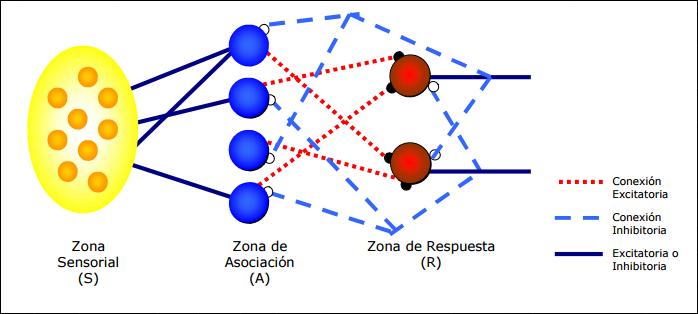
\includegraphics[width=0.95\textwidth]{Fotoperceptron.PNG}
\caption{Fotoperceptron}
\label{Fotoperceptron}
\end{figure}

\begin{itemize}
    \item La luz incide en los puntos sensibles $(S)$ de la estructura de la retina y cada uno de esos puntos responde en forma todo-nada a la luz entrante.
    \item Los impulsos generados por $(S)$ se transmiten a las unidades de asociación $(A)$, donde cada unidad de $(A)$ está conectada a un conjunto aleatorio de puntos de $(S)$. Estas conexiones tienen los valores posibles $+1$, $-1$ y $0$.
    \item Cuando aparece un conjunto de estímulos en la retina $(S)$, una unidad de $(A)$ se activa si la suma de sus entradas sobrepasa algún valor umbral. Si la unidad esta activada, produce una salida que se envía a la siguiente capa de unidades.
    \item De forma similar, las unidades de $(A)$ están conectadas a unidades de respuesta $(R)$ y la conectividad vuelve a ser aleatoria entre ellas.
\end{itemize}

Se pudo demostrar que el Perceptrón era capaz de clasificar patrones correctamente, en lo que Rosenblatt denominaba un entorno diferenciado, en el cual cada clase estaba formada por patrones similares. El Perceptrón también era capaz de responder de manera congruente frente a patrones aleatorios, pero su precisión iba disminuyendo a medida que aumentaba el número de patrones que intentaba aprender.

En 1969 Marvin Minsky y Seymour Papert publicaron su libro: "Perceptrons: An introduction to Computational Geometry", en el que se presentaba un análisis detallado del Perceptrón, en términos de sus capacidades y limitaciones. La mayor desventaja de este tipo de redes es su incapacidad para solucionar problemas que no sean linealmente separables.

Minsky y Papert se apartaban de la aproximación probabilística de Rosenblatt y volvían a las ideas de cálculo de predicados en el análisis del Perceptrón.

La estructura de un Perceptrón sencillo es similar a la siguiente:

\begin{figure}[H]
\centering
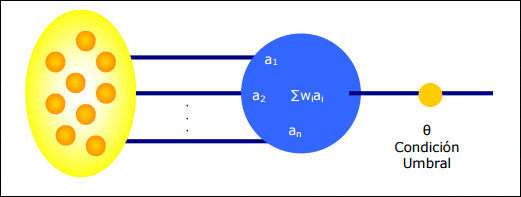
\includegraphics[width=0.7\textwidth]{Perceptron.PNG}
\caption{Estructura Perceptron}
\label{Estructura Perceptron}
\end{figure}

en la cual se observa la adición de una condición umbral en la salida. Si la entrada completa a esta condición es mayor que el valor umbral, la salida de la red es $1$ y en caso contrario es $-1$.

De manera más específica, el Perceptrón se puede definir de la manera siguiente:

\textit{Un \textbf{perceptrón simple} es un dispositivo de computación con umbral $\theta$ y $N$ entradas reales $x_1, ..., x_N$ a través de arcos con pesos $w_1, ..., w_N$ y que tiene salida $1$ cuando $\sum_{i}w_ix_i \geq \theta$ y $-1$ en caso contrario.}

Es decir, supongamos la función  de clasificación $f$ en $\mathbb{R}^n$ tal que:

\[
f(x_1, x_2, ..., x_N) = \left\{ \begin{array}{lcc}
             1 &   si  & w_1x_1 + w_2x_2 + ... + w_Nx_N \geq \theta \\
             \\ -1 &  si  &  w_1x_1 + w_2x_2 + ... + w_Nx_N < \theta 
             \end{array}
   \right.
\]

Dicha función realiza una partición en el espacio $\mathbb{R}^n$ de patrones de entrada: por una parte estarían los patrones con salida $+1$ y por otra parte los patrones con salida $- 1$. Por lo tanto, diremos que la función f clasifica a los patrones de entrada en dos clases.

En este caso, se expresa la función $f$ mediante la función signo, es decir:
\[
f(x_1, x_2, ..., x_N) = sign(x_1, x_2, ..., x_N)
\]

donde la función signo es:
\[
sign(x_1, x_2, ..., x_N) = \left\{ \begin{array}{lcc}
             1 &   si  & x \geq 0 \\
             \\ -1 &  si  &  x < 0 
             \end{array}
   \right.
\]

El algoritmo de aprendizaje del perceptrón consiste en lo siguiente:
\begin{enumerate}
    \item Suponemos que el conjunto de datos es linealmente separable y que se puede encontrar una solución correcta del problema.
    \item El objetivo será buscar el vector $W$ (tal que su hiperplano asociado separe los puntos) que alcanza la solución correcta para todos los puntos.
    \item Suponemos unas salidas esperadas prefijadas $Y_i$ para cada punto a clasificar (con valores $+1$ y $-1$).
    \item \textbf{Paso 1:} Elegir un punto $X_i$ y seleccionar el vector $W_i$ de los pesos en ese momento (al principio dicho vector se podrá inicializar a $0$). Es decir, tenemos las parejas siguientes: ${(X_1, Y_1), ..., (X_N, Y_N)}$ y el algoritmo cogerá un punto que está mal clasificado en ese momento.
    \item \textbf{Paso 2 y sucesivos:} Para el punto $X_i$ seleccionado actualmente, calcular $sign(W^T \times X_i)$.
    \begin{itemize}
        \item Si $sign(W^T \times X_i) \neq Y_i \Rightarrow$ aplicar la regla de actualización $W_{i+1} = W_i + Y_iX_i$.
        \item En caso contrario, volver al paso 2 y continuar el algoritmo con el siguiente punto.
    \end{itemize}
    \item La regla de adaptación de pesos del Perceptrón realiza un movimiento en la dirección correcta para clasificar bien el punto actual $X_i$.
    \item El algoritmo finaliza cuando no haya más puntos mal clasificados.
\end{enumerate}

\begin{figure}[H]
\centering
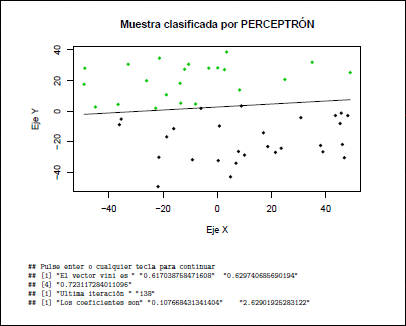
\includegraphics[width=0.9\textwidth]{ejemploPerceptron.PNG}
\caption{Ejemplo Perceptron}
\label{Ejemplo Perceptron}
\end{figure}
 
\subsection{Nearest Neighbor}
El algoritmo de clasificación \textbf{K-Nearest Neighbour (k-NN)} o \textbf{K-Vecino más Cercano} es uno de los métodos de clasificación más fundamentales y sencillos, y debería ser una de las primeras opciones para un estudio de clasificación cuando hay poco o ningún conocimiento previo sobre la distribución de los datos.

Este algoritmo de clasificación se desarrolló debido a la necesidad de realizar análisis discriminantes (que es una técnica estadística capaz de decirnos qué variables permiten diferenciar distintos grupos y cuántas de estas variables son necesarias para alcanzar la mejor clasificación posible) cuando las estimaciones paramétricas fiables de las densidades de probabilidad son desconocidas o difíciles de determinar.

En 1951, \textbf{Fix y Hodge} introdujeron este método no paramétrico para la clasificación de patrones, conocido desde aquel entonces como la regla del k-vecino más cercano.

Pero no fue hasta el año \textbf{1967} cuando se tuvo constancia de este método y se resolvieron algunas de las propiedades formales de dicho algoritmo. Por ejemplo, se demostró que para $k = 1$ y $n \rightarrow \infty$ el error de clasificación de este algoritmo está delimitado por dos veces la tasa del error de Bayes \textit{(Cover \& Hart, 1967)}.

Por ello, y de manera resumida, se dice que en 1967, Fix \& Hodge desarrollan el algoritmo \textbf{Nearest Neighbour} o \textbf{Vecino más Cercano}.

Este hito está considerado como el nacimiento del \textit{campo del reconocimiento de patrones} o \textit{pattern recognition} en computadores.

Una vez que se establecieron en 1967 tales propiedades formales, se siguió una larga línea de investigación incluyendo nuevos enfoques de rechazo \textit{(Hellman, 1970)}, refinamientos con respecto a la tasa de error de Bayes \textit{(Fukunaga y Hostetler, 1975)}, enfoques basados en la distancia \textit{(Dudani, 1976; Bailey y Jain, 1978)}, soft computing \textit{(Bermejo y Cabestany, 2000)} y métodos difusos \textit{(Jozwik, 1983; Keller et al., 1985)}.

Los primeros programas capaces de reconocer patrones fueron diseñados en base a este algoritmo.

Dicho algoritmo se basa en:
\begin{itemize}
    \item \underline{El aprendizaje basado en casos}: extracción de información de un conjunto de datos conocidos para clasificar nuevos o agrupar existentes.
    \item \underline{El razonamiento basado en casos}: imitación del sentido común humano a través de experiencias pasadas y solución de problemas presentes con analogías de problemas pasados.
    \item \underline{Métodos basados en vecindad y de medición de distancia}.
\end{itemize}

Las aplicaciones más importantes de este algoritmo son:
\begin{enumerate}
    \item Escalamiento de gráficos evitando la menor pérdida de píxeles.
    \item Sistemas de GPS actuales.
    \item Reconocimiento de rostros.
\end{enumerate}

\textbf{¿Cómo funciona k-NN?}
Parte de la idea de que una nueva muestra será clasificada en la clase a la cual pertenezcan la mayor cantidad de vecinos más cercanos (del conjunto de entrenamiento más cercano) a esta.

Es decir, cuando se le da un nuevo objeto al programa, éste lo compara con los datos del conjunto de entrenamiento y clasifica el objeto con el vecino más cercano o con el objeto más similar en la memoria.

Veamos un ejemplo del funcionamiento de esta regla de clasificación:
\begin{shaded}
Representamos 12 muestras pertenecientes a dos clases distintas: la Clase 1 está formada por 6 cuadrados de color azul y la Clase 2 está formada por 6 círculos de color rojo.

Seleccionamos tres vecinos, es decir, $k = 3$.

De los $3$ vecinos más cercanos a la muestra $x$ (representada en la figura por una cruz) uno de ellos pertenece a la Clase 1 y los otros dos a la Clase 2.

Por tanto, la regla $3-NN$ asignará la muestra $x$ a la Clase 2.
\end{shaded}

\begin{figure}[H]
\centering
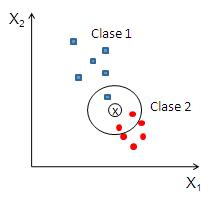
\includegraphics[width=0.5\textwidth]{ejemploKNN.JPG}
\caption{Ejemplo kNN}
\label{Ejemplo kNN}
\end{figure}

\begin{shaded}
Es importante señalar que si se hubiese utilizado como regla de clasificación la $1-NN$, la muestra $x$ sería asignada a la Clase 1, pues el vecino más cercano de la muestra $x$ pertenece a la Clase 1.
\end{shaded}

\subsection{Otros algoritmos que clasifican}
\subsubsection{Árboles de decision}
Un \textbf{árbol de decisión} es un grafo dirigido donde los nodos son reglas sobre los atributos del conjunto de instancias y las hojas del árbol son el atributo clase o el atributo sobre el que se va a intentar clasificar. A lo largo de la historia se han ido surgiendo algoritmos que siguen esta estructura con el objetivo de dar una solución al problema de la clasiificación, algunos de los algoritmos más relevantes que aprenden basandose en árboles de decisión son:
\begin{itemize}
\item \textbf{Algoritmo ID3:} Es un algoritmo que indice árboles de decisión a partir de un conjunto dado de instancias con atributos determinados, fue inventado por \textbf{John Ross Quinlan} en los años 60 siguiendo el sencillo principio de la \textbf{navaja de Occam} para intentar construir un árbol de decisión lo más pequeño posible.

El algoritmo trata de calcular la entropía o valor promedio que cada uno de los atributos de un conjunto de datos y haciendo uso de esta información dividir en subconjuntos más pequeños basandose en las instancias con la entropía mínima o máxima dependiendo del criterio, para despues construir un árbol de decisión que contenga el atributo con dicha entropía, a partir de aqui utiliza la recursividad para repetir el proceso con los demás atributos.
\item \textbf{Algoritmo C4.5:} Es el precursor del algoritmo ID3 desarrollado también por Quinlan que empezo a tomar relevancia despues de que obtubiera el primer puesto  en el documento publicado por Springer LNCS llamado \textit{''Top 10 Algorithms in Data Mining''}.
El algoritmo construye árboles de decisión de la misma manera que lo hace el algoritmo ID3 usando el concepto de entropía solo que ahora el criterio de selección de que atributo usar para dividir el conjunto en subconjuntos de forma efectiva cambia usandose una ganancia de información o entropía relativa, esta medida es la diferencia entre dos distribuciones de probabilidad P y Q donde P representa la distribución de valores corectamente clasificados y Q  es una aproximación de P.
\item \textbf{Algoritmo Random Forest:} Recientemente en el año \textbf{1995}, \textbf{Tinkam Ho} un analísta de datos publica un documento en el que se describia este algoritmo, este algoritmo trata de construir un conjunto de árboles de decisión. Haciendo uso de un conjunto de entrenamiento hacemos que se construya un conjunto de árboles de decisión en el que dada una entrada, que puede ser una nueva instancia, esta se clasifica por todos los árboles del conjunto y se predice a que clase esta instancia pertenece en función de la mayoría de los resultados de la clasificación anterior, es decir si hay 3 árboles de decisión y 2 dicen que pertenece a el conjunto de instancias mal clasificadas entonces ese será su valor de clase.
\end{itemize}
\subsubsection{Support Vector Machine}
El algortimo \textbf{support vector machine} o SVM son un conjunto de \textbf{técnicas de aprendizaje supervisado} desarrollados por publicado en un documento en el año \textbf{1995} en el que trabajaron \textbf{Corinna Cortes} y \textbf{Vladimir Vapnik}, es un método que dado un conjunto de entrenamiento construye un modelo que servirá para realizar predicciones sobre un conjunto de instancias o una muestra del mismo tipo. Es un modelo que representa las instancias en el espacio separando las clases lo máximo haciendo uso de un hiperplano o un conjunto de hiperplanlos dependiendo de la dimensionalidad de los atributos del conjunto de datos la idea es que estos  separen de forma óptima las clases. Este algoritmo puede ser usado tanto en problemas de regresión como en problemas de clasificación. 

Este algoritmo pertenece a la familia de clasificadores lineales, es decir, algoritmos que tratan de clasificar una instancia basandose en valores de una combinación lineal de sus atributos.

\section{Máquinas y juegos}
En esta sección mencionaremos los años y nombraremos las personalidades que han sido capaces de crear un programa o programas basandose en algoritmos de aprendizaje para que las máquinas sean capaces de aplicar las reglas del juego de una forma lógica y siempre con la intención de ganar.
\subsection{Máquinas jugando a las Damas}
En el año \textbf{1952} \textbf{Arthur Samuel }que acababa de unirse a un laboratorio de investigación de IBM escribe uno de los primeros programa de aprendizaje automático capaz de jugar a las damas. Se le denomina como un pionero en el campo de juegos de ordenador e inteligencia artificial. El programa de Samuel parece que fue el \textbf{"primer programa"} en el mundo capaz de aprender.

\begin{figure}[H]
\centering
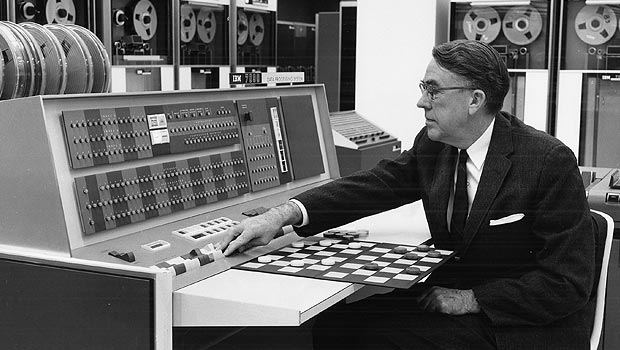
\includegraphics[width=0.5\textwidth]{acc}
\caption{Arthur Samuel jugando a las damas}
\label{Ejemplo kNN}
\end{figure}

El programa hacía uso de un árbol de juegos basandose en la estrategia minimax principalmente y usando la poda $\alpha\beta$ algoritmos que tratan de anticiparse a lo que hará el contrincante generando un árbol de acciones y podando quedandose con los caminos más probables y eligiendo aquel que obtenga un mayor porcentaje de victoria, pero luego diseñó varios mecanismos que le permitirían mejorar su programa, a estos mecanismos los denomino rote learning o aprendizaje por rutina que es básicamente una técnica que recuerda cada una de las posiciones que ya han sido visitadas basandose en la repeteción y una revaloración del estado de juego.

\subsection{Máquinas jugando al Backgammon}
En el año \textbf{1992}, \textbf{Gerry Tesauro} desarrolla un programa de aprendizaje capaz de jugar al backgammon, basandose en conocimiento obtenido del juego. Esta aplicación del aprendizaje automático fue capaz de jugar casi tan bien como el campeón mundial en el juego. El aprendizaje estaba basado en un algoritmo abreviado TD o temporal difference learning, es un algortimo que trata de realizar predicciones basado en una combinación del método de Monte Carlo y la programación dinámica.

\subsubsection{Máquinas jugando al Ajedrez}

\begin{figure}[H]
\centering
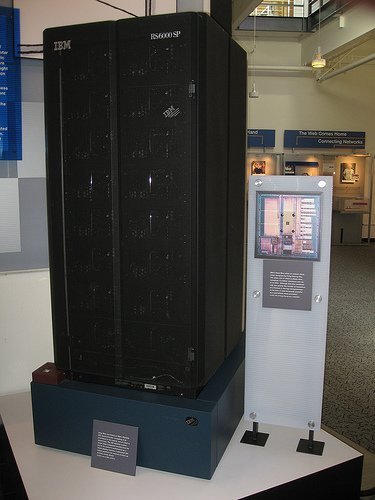
\includegraphics[width=0.5\textwidth]{deepblue}
\caption{Máquina Deep Blue de IBM}
\label{Ejemplo kNN}
\end{figure}

La supercomputadora \textbf{Deep Blue} instalada el año \textbf{1996} y desarrollada por IBM era capáz de jugar al ajedrez, lo novedoso de esto es que fue la primera máquina que consiguió vencer una partida al vigente campeón del mundo \textbf{Gary Kasparov} en un encuentro de 6 partidas realizado el mismo año. Sin embargo deep blue no fue capaz de ganar el encuentro debido a que Kasparov gano 4 de los 6 y empató los otros 2. En el año \textbf{1997} esta máquina tuvo una considerable mejora pasandose a llamar Deeper Blue que volvio a jugar contra aún vigente campeón del mundo Kasparov de nuevo en un encuentro a 6 partidas donde esta vez ganó \textbf{Deeper blue} con 3 victorias 2 derrotas y 1 empate.

\subsection{Máquinas jugando al go}

En el año \textbf{2015 Google DeepMind} de Londres desarrolla un programa de ordenador llamado AlphaGo capaz de jugar al juego Go. Que resulta ser el primer programa que juega a ese juego en derrotar una persona profesional en un tablero de 19x19. El juego Go es considerado mucho más dificil de tratar computacionalmente que otros juegos como el ajedrez debido a que se tiene una gran cantidad de opciones y por tanto un gran árbol de decisión generado. Esto hace que los típicos algoritmos como la poda $\alpha\beta$ y otros métodos de búsqueda sean difíciles de usar, la capacidad de aprendizaje del programa se basa en una red neuronal que usa deep learning. El deep learning es una rama del machine learning que toma un conjunto de algoritmos que intentan obtener un modelo de abstracciones sobre los datos.

\section{Stanford cart y otros experimentos}
El \textbf{Stanford Cart} nació de una investigación para controlar un Moon Rover desde la Tierra. Fue construido en \textbf{1960} por un estudiante, \textbf{James L. Adams}, quien había estado trabajando en un proyecto de la NASA que pretendía que alguien desde la Tierra pudiese conducir alrededor de la Luna usando una cámara de vídeo en el vehículo.
Adams se centró en estudiar la controlabilidad del vehículo con varias configuraciones de la velocidad de comunicación. Demostró que con un retardo de comunicación correspondiente al viaje de ida y vuelta a la Luna (aproximadamente 2.5 segundos), el vehículo no podía ser controlado de manera fiable si viajaba a más de 0.3 km/h.

En \textbf{1962} otro estudiante, \textbf{Paul W. Braisted}, ideó un esquema para mejorar la controlabilidad del vehículo agregando una computadora que funcionaba como un predictor que tomaba en cuenta comandos de dirección anteriores y dibujaba un punto en la pantalla de televisión que indicaba la localización cuando una orden se llevara a cabo. Con esta mejora el vehículo podría ser controlado a 8 km/h. 

En \textbf{1969}, \textbf{Lester Earnest} intentó construir un vehículo de carretera auto-dirigido basado en el aporte visual. Earnest tenía en mente tratar de conducir por la carretera circular que rodea la instalación de SAIL usando la línea central del camino y otras referencias visuales. Sin embargo sabía que el carro no podría llevar una computadora bastante grande para hacer eso, así que planeó utilizar un transmisor en el carro para enviar imágenes de la cámara de la TV a la computadora y otro enlace de radio para enviar órdenes de guía de la computadora al carro. Las operaciones experimentales comenzaron con un operador humano que controlaba el carro a través de la computadora usando imágenes de televisión. Utilizando el procesador KL10 entonces disponible, que funcionaba a unos 2,5 MIPS, \textbf{Hans Moravec} fue capaz de usar la visión multi-ocular para navegar lentamente alrededor de los obstáculos en un ambiente interior.
En \textbf{1979}, el carro cruzó con éxito una sala llena de sillas sin intervención humana en unas cinco horas.
\begin{figure}[H]
	\centering
	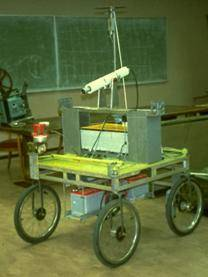
\includegraphics[width=0.5\textwidth]{stanford_cart.jpg}
	\caption{Stanford Cart}
	\label{Stanford Cart}
\end{figure}
Hoy en un día hay varios programas activos de investigación para fabricar coches completamente autónomos.En agosto de 2016 la empresa estadounidense nuTonomy, filial del MIT, lanzó el primer taxi autónomo del mundo en Singapur.
\section{Neocognitron}
El neocognitron es una red neuronal artificial jerárquica y multicapa propuesta por \textbf{Kunihiko Fukushima} en los años ochenta.Se ha usado para el reconocimiento de caracteres escritos a mano y otras tareas de reconocimiento de patrones, y sirvió de inspiración para redes neuronales convencionales.Su diseño se basó en el trabajo anterior realizado por Hubel y Weisel que aclaraba parte de la arquitectura funcional de la corteza visual.

El neocognitron consiste en múltiple tipos de células, las más importantes son las llamadas células S y células C. Las células S funcionan como células que extraen características. Sus conexiones de entrada son variables y se modifican a través del aprendizaje. En términos generales, las características locales, tales como bordes o líneas en orientaciones particulares, se extraen en etapas inferiores. Más características globales, como partes de los patrones de aprendizaje, se extraen en etapas superiores.
Las células C, se insertan en la red para permitir errores de posición en las características del estímulo. Cada célula C recibe conexiones de entrada excitatoria de un grupo de células S que extraen la misma característica, pero desde posiciones ligeramente diferentes. La célula C responde si al menos una de estas células S produce una salida.

\begin{figure}[H]
	\centering
	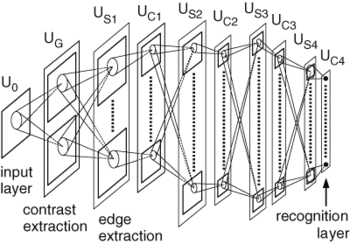
\includegraphics[width=0.5\textwidth]{neocognitron1.png}
	\caption{Estructura del neocognitron.}
	\label{Estructura del neocognitron.}
\end{figure}

\subsection{Final con el estado actual del machine learning}
Esto va a ser una recopilación de los finales que encontreis para cada área.
\begin{thebibliography}{9}

 \bibitem{Timeline}
 \url{https://en.wikipedia.org/wiki/Timeline_of_machine_learning}

\bibitem{articulointro}
 	\textbf{Introducción},
 \url{http://cleverdata.io/que-es-machine-learning-big-data/}
 
 \bibitem{conceptosbasicos}
 	\textbf{Introducción},
 \url{ftp://decsai.ugr.es/pub/usuarios/castro/Actividades/Redes-Neuronales/Apuntes/Apuntes%20Javier%20Rodriguez%20Blazquez/Conceptos%20basicos.pdf}

\bibitem{estadistica1}
\url{http://www.centrodeinnovacionbbva.com/noticias/las-cinco-tribus-del-machine-learning}

\bibitem{standford1}
	\textbf{Neural Networks},
  \url{http://cs.stanford.edu/people/eroberts/courses/soco/projects/neural-networks/History/history2.html}
 
 \bibitem{standford2}
 	\textbf{Neural Networks},
 \url{http://cs.stanford.edu/people/eroberts/courses/soco/projects/neural-networks/History/history1.html}
 
 \bibitem{wikiNN1}
 	\textbf{Neural Networks},
 \url{https://en.wikipedia.org/wiki/Artificial_neural_network}
 
 \bibitem{marvinminsky}
 	\textbf{Neural Networks},
 \url{https://en.wikipedia.org/wiki/Marvin_Minsky}
 
 \bibitem{historiademachinelearning}
 	\textbf{Perceptrón},
 \url{http://sge.wonderville.ca/machinelearning/history/history.html}
 
 \bibitem{perceptron1}
 	\textbf{Perceptrón},
 \url{http://www.lcc.uma.es/~jmortiz/archivos/Tema4.pdf}
 
 \bibitem{perceptron2}
 	\textbf{Perceptrón},
 \url{ftp://decsai.ugr.es/pub/usuarios/castro/Actividades/Redes-Neuronales/Apuntes/Apuntes%20Javier%20Rodriguez%20Blazquez/Redes%20de%20una%20capa.pdf}
 
  \bibitem{neighbour1}
 	\textbf{Nearest Neighbour},
 \url{http://sge.wonderville.ca/machinelearning/history/history.html}
 
 \bibitem{neighbour2}
 	\textbf{Nearest Neighbour},
 \url{http://www.synergicpartners.com/una-breve-historia-del-machine-learning/}
 
 \bibitem{neighbour3}
 	\textbf{Nearest Neighbour},
 \url{http://www.scholarpedia.org/article/K-nearest_neighbor}
 
 \bibitem{neighbour4}
 	\textbf{Nearest Neighbour},
 \url{http://todobi.blogspot.com.es/2016/02/una-breve-historia-del-machine-learning.html}
 
 \bibitem{neighbour5}
 	\textbf{Nearest Neighbour},
 \url{https://prezi.com/0oyoj6v-eycs/algoritmo-knn/}
 
 \bibitem{neighbour6}
 	\textbf{Nearest Neighbour},
 \url{https://www.ecured.cu/Regla_de_los_K_vecinos_m%C3%A1s_cercanos}
 
 \bibitem{neighbour7}
 	\textbf{Nearest Neighbour},
 \url{https://prezi.com/lzilzh3g8xvf/algoritmo-de-los-k-vecinos-mas-proximos/}
 
  \bibitem{turing1}
 	\textbf{Máquina de aprendizaje de Turing},
 \url{https://hipertextual.com/2011/10/inteligencia-artificial-test-de-turing}
 
 \bibitem{turing2}
 	\textbf{Máquina de aprendizaje de Turing},
 \url{http://matap.dmae.upm.es/cienciaficcion/DIVULGACION/3/TestTuring.htm}
 
 \bibitem{turing3}
 	\textbf{Máquina de aprendizaje de Turing},
 \url{https://es.wikipedia.org/wiki/Test_de_Turing}
 
 \bibitem{turing4}
 	\textbf{Máquina de aprendizaje de Turing},
 \url{http://xamanek.izt.uam.mx/map/cursos/Turing-Pensar.pdf}
 
 \bibitem{turing5}
 	\textbf{Máquina de aprendizaje de Turing},
 \url{http://enciclopedia.us.es/index.php/Prueba_de_Turing}
 
    \bibitem{stanford}
    \textbf{Stanford Cart},
    \url{http://web.stanford.edu/~learnest/sail/cart.htm}
 \bibitem{neocognitron1}
 \textbf{Neocognitron},
 \url{https://en.wikipedia.org/wiki/Neocognitron}
 \bibitem{neocognitron2}
 \textbf{Neocognitron},
 \url{http://www.scholarpedia.org/article/Neocognitron}
\end{thebibliography}
\end{document}